\begin{figure*}[t]
\centering
{\sffamily
\setlength{\tabcolsep}{4pt}
(a) \begin{tabular}{c|c|c|c|c|c|c|c}
\texttt{\#78} (284 nt) & Boltzmann & & struct. & energy gap & & & \\
``Mat - Lot 2-2 B'' & prob.\ $(\uparrow)$ & \NED$(\downarrow)$ & dist.\ $(\downarrow)$ & (kcal/mol) $(\downarrow)$ & \MFE & uMFE & designable \\
\hline
EliteDesign ($N=500$) & \textbf{0.0073} & \textbf{0.042} & \textbf{4} & \textbf{2.4} & No & No & \multirow{2}{*}{No} \\
SamplingDesign & 0.000235 & 0.157 & \textbf{4} & 3.3 & No & No & \\
\hline
Probability ceiling & 0.0184 & --- & --- & --- & --- & --- & --- \\
\end{tabular}}\\[4pt]
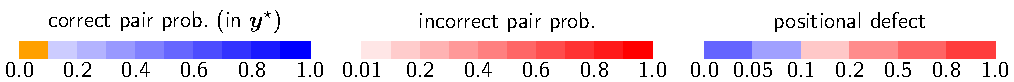
\includegraphics[width=0.85\linewidth]{figures/structures/legend}\\[2pt]
{\sffamily
\begin{tabular}{@{}c@{\hspace{0.02\linewidth}}c@{\hspace{0.02\linewidth}}c@{}}
(b) Target \vecystar & (c) \MFE of EliteDesign ($N=500$) & (d) \MFE of SamplingDesign \\[2pt]
\raisebox{-0.5\height}{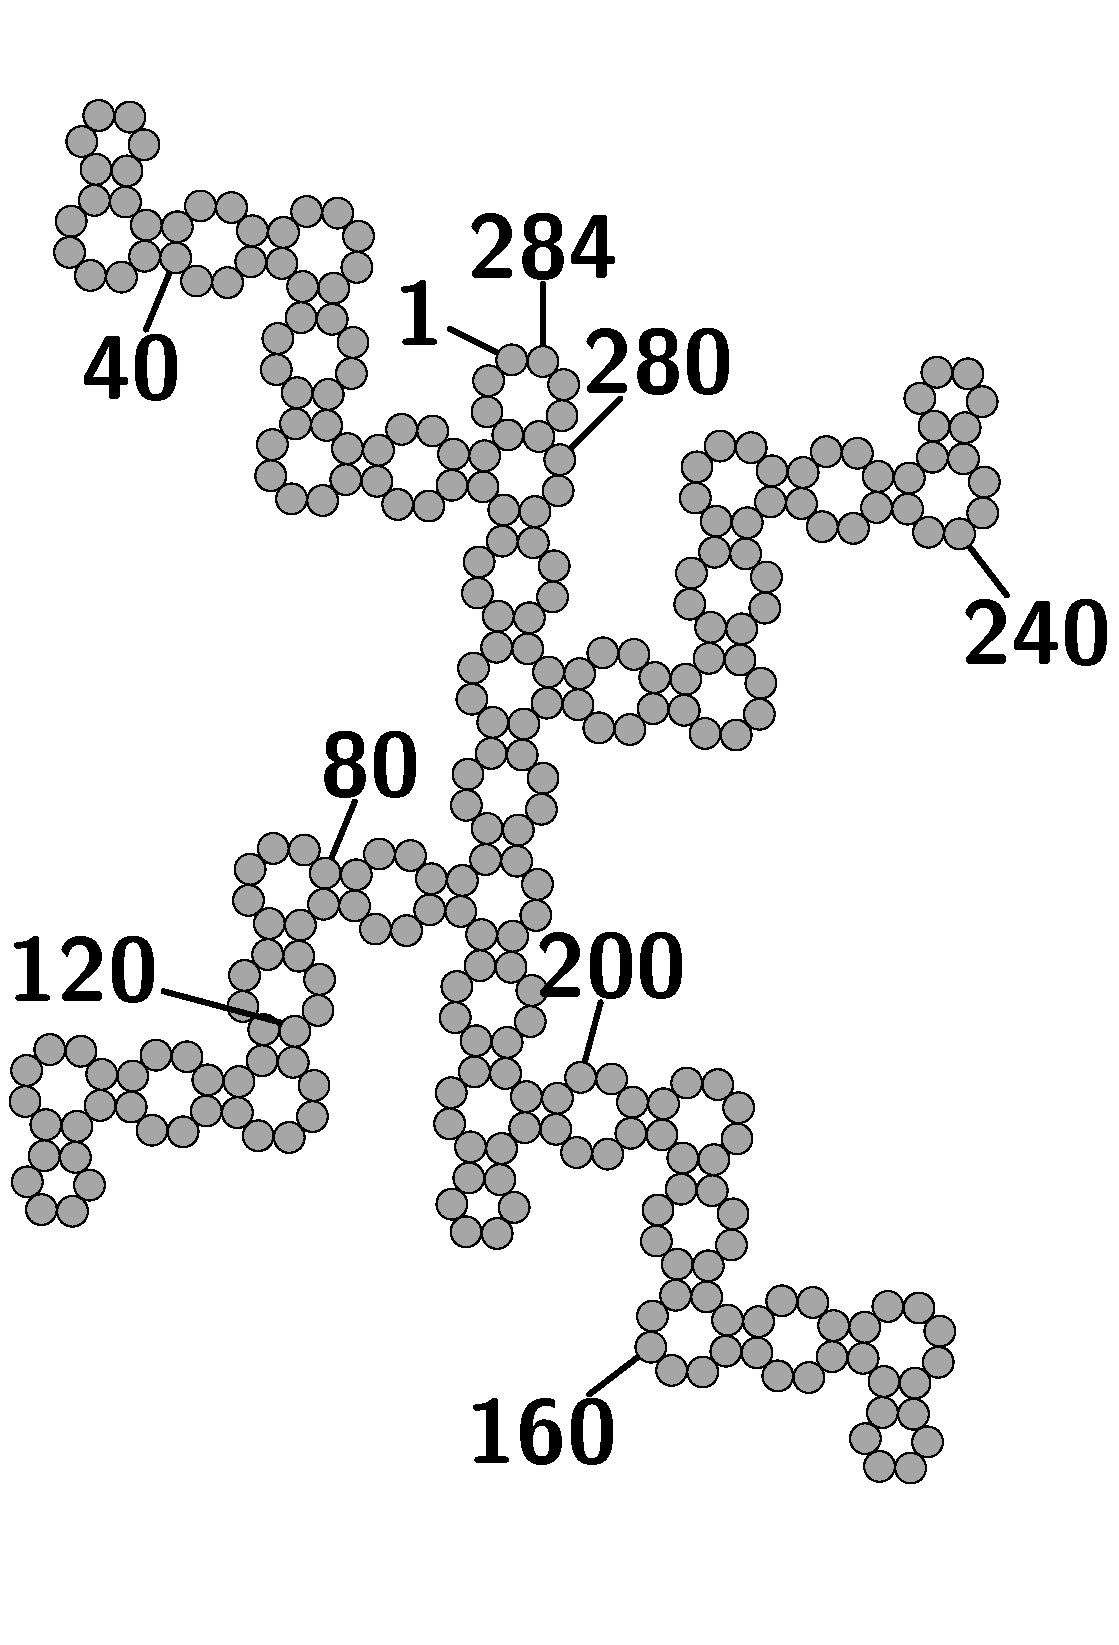
\includegraphics[width=0.195\linewidth,trim=0 75 3 45,clip]{figures/structures/target_78_big}} &
\raisebox{-0.5\height}{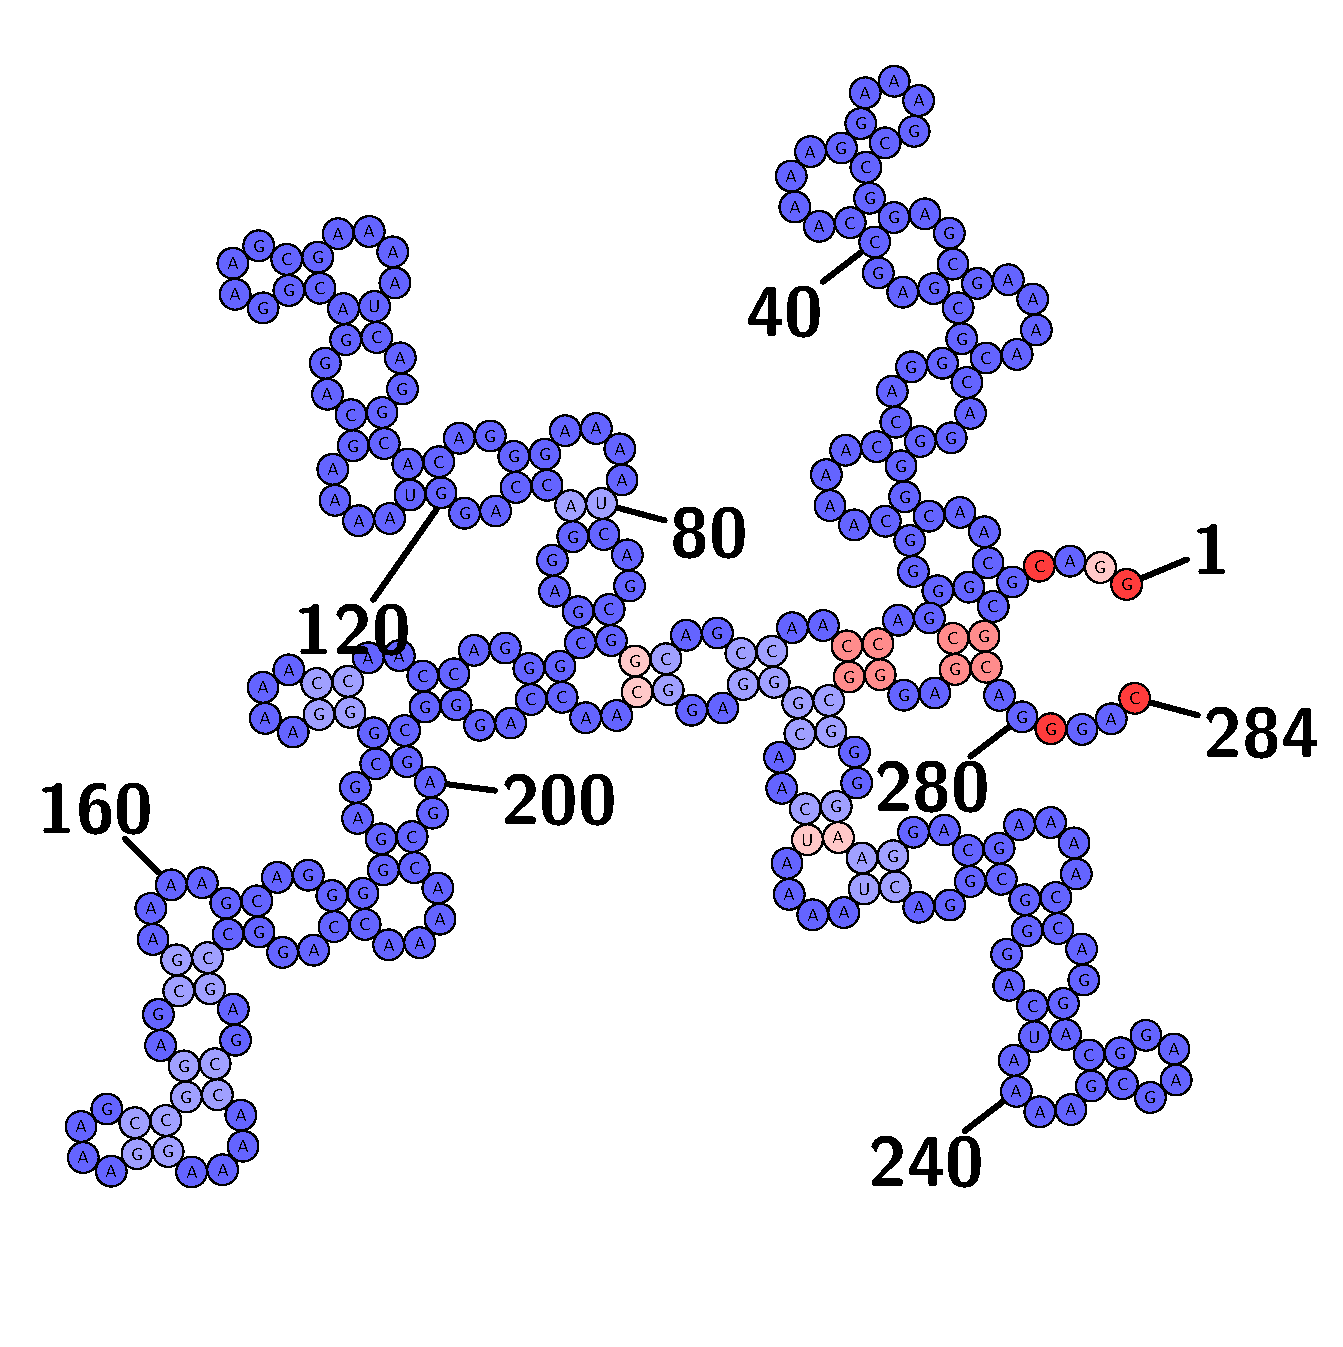
\includegraphics[width=0.37\linewidth,trim=18 74 10 29,clip]{figures/structures/structure_78_elite_big}} &
\raisebox{-0.5\height}{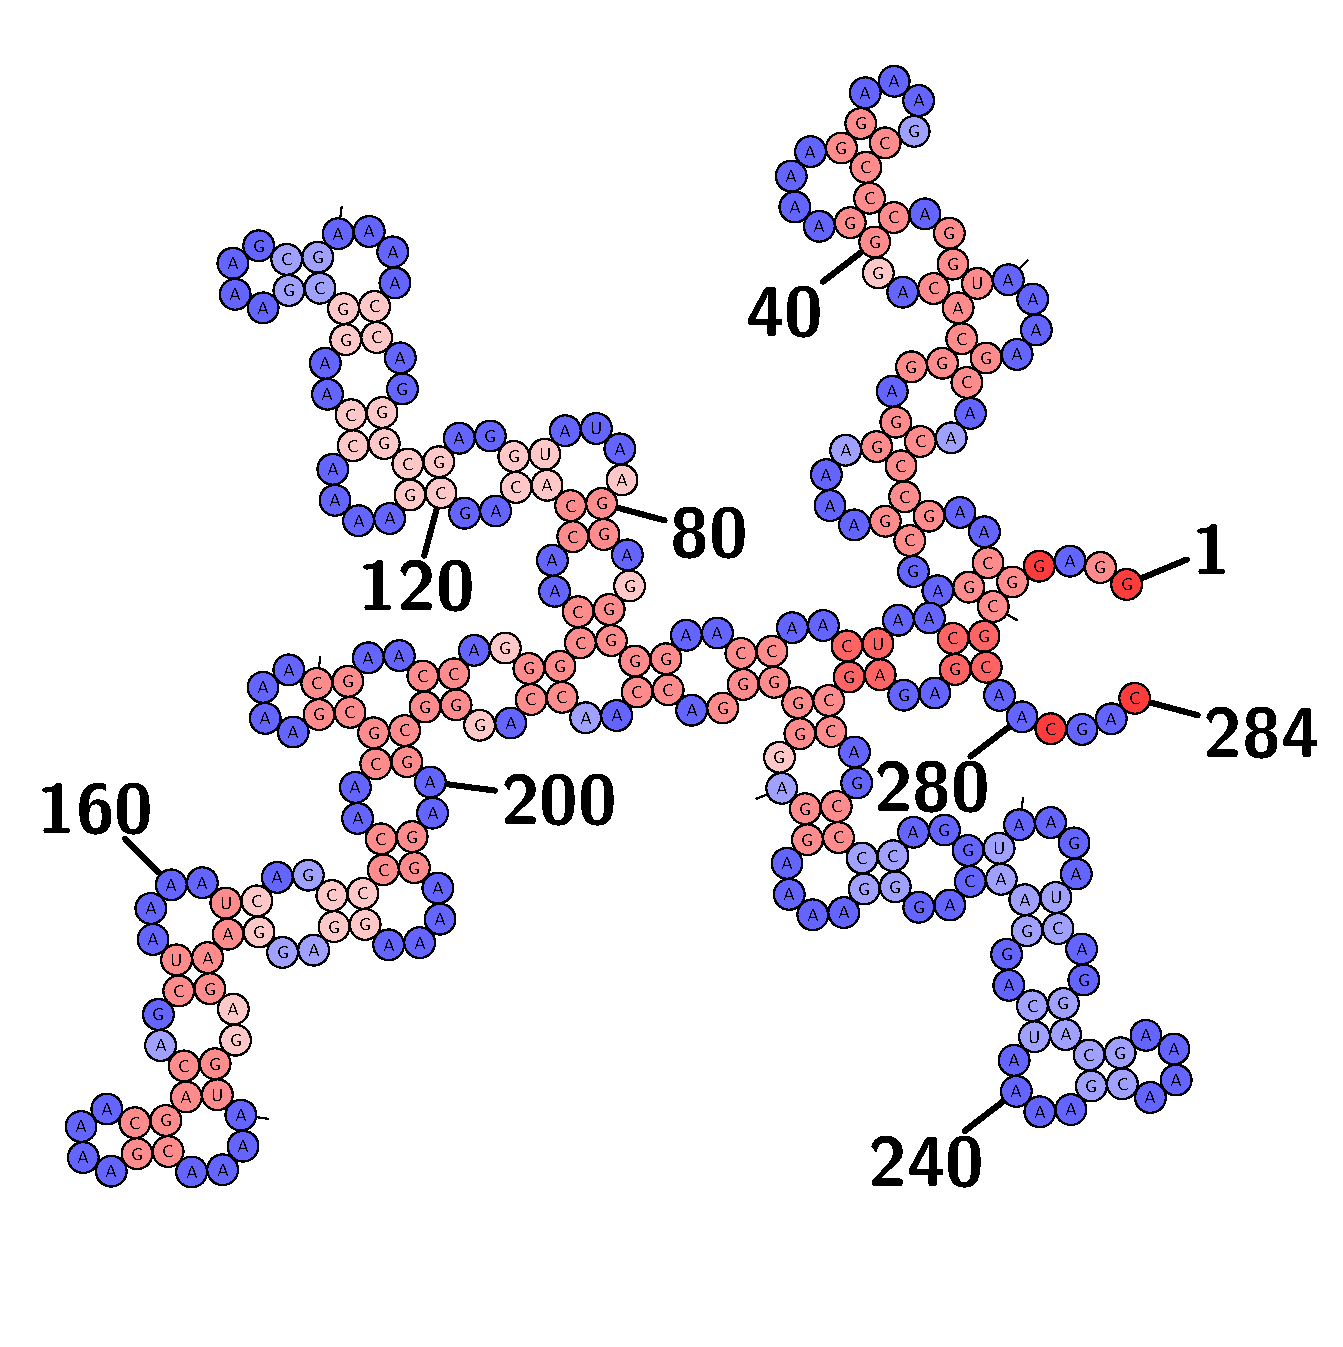
\includegraphics[width=0.37\linewidth,trim=18 74 10 29,clip]{figures/structures/structure_78_sampling_big}}
\end{tabular}\\[4pt]
\begin{tabular}{@{}c@{\hspace{0.03\linewidth}}c@{}}
(e) Base-pairing probabilities, EliteDesign ($N=500$) & (f) Base-pairing probabilities, SamplingDesign \\[1pt]
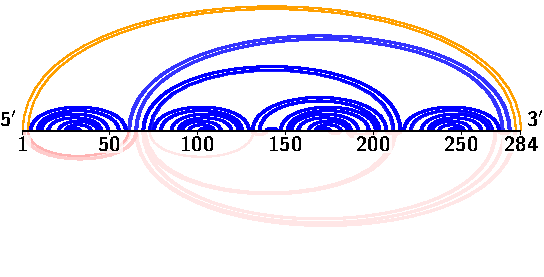
\includegraphics[width=0.46\linewidth,trim=0 8 0 0,clip]{figures/structures/arcs_78_elite_big} &
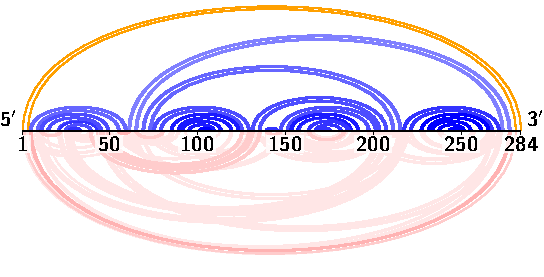
\includegraphics[width=0.46\linewidth,trim=0 8 0 0,clip]{figures/structures/arcs_78_sampling_big}
\end{tabular}}
\caption{The sequences with the highest Boltzmann probability from EliteDesign ($N=500$) and SamplingDesign on Puzzle \texttt{\#78} (``Mat - Lot 2-2 B'', 284 nucleotides), which is proven undesignable. The panels and colors are as in Fig.~\ref{fig:eterna-structure-90}.}
\label{fig:eterna-structure-78}
\end{figure*}
